\documentclass[12pt]{article}

\usepackage{geometry}
\usepackage[utf8]{inputenc}
\usepackage[T2A]{fontenc}
\usepackage[russian]{babel}
\usepackage{graphicx}
\usepackage{caption}
\usepackage{amssymb, gensymb, amsmath}
\usepackage{mathrsfs}
\usepackage{array, colortbl}
\usepackage{multicol}

\title{{\bf Лабораторная работа 5.\, 1. \\ Измерение коэффициента ослабления $\gamma$-лучей в веществе и определение их энергии}}
\author{Лось Денис (группа 618)}
\date{9 ноября 2018}

\begin{document}

\maketitle

\paragraph*{Цель работы: } с помощью сцинтилляционного счетчика измерить линейные коэффициенты ослабления потока $\gamma$-лучей в свинце, железе и алюминии; по их величине определить энергию $\gamma$-квантов.

\section*{Введение в теоритическую часть}
\par
	Ослабление интенсивности потока лучей в веществе:
\begin{align*}
	I &= I_0 \cdot e^{-\mu l} \\
	I &= I_0 \cdot e^{-\mu' m} \\
\end{align*}
\par
	Выражение для коэффициента ослабления:
\[
	\mu = \frac{1}{l} \ln \frac{N}{N_0}
\]
\par
	Значения $N$ и $N_0$ определеляются с учётом поправок, вносимых фоном.
\begin{align*}
	N_0 &= n_0 - n_\text{фон} \\
	N &= n - n_\text{фон} \\
\end{align*}

\section*{Ход работы и результаты исследования}
\subsection*{Определение фона}
\par
	Проведём измерения фона с помощью заглушки и длинного металлического цилиндра

\begin{table}[h!]
	\centering
	\begin{tabular}{|c|c|c|c|c|}
	\hline
		Образец & Длина образца $l$, см & $N$ & $\Delta N$ & $t$, c \\
	\hline
		Цилиндр & 19 & 1753 & 42 & 100 \\
	\hline
		Заглушка & 7 & 1901 & 44 & 100 \\ 
	\hline
	\end{tabular}
\end{table}

\par
	Несмотря на получившиеся различия в определения фона различными методами, поправку на фон будем делать по измерениям, проведённым с помощью заглушки.

\subsection*{Исследование поглощения $\gamma$-квантов в различных образцах}
\par
	Исследуем поглощение $\gamma$-лучей в свинце, железе и алюминии. Из полученных результатов построим график для определения коэффициента ослабления.

\paragraph*{Исследование для железа: }
\par
	Число частиц, попадающих в счётчик в отсутствие поглотителя $N_0$ (с учётом фона):
\[
	N_0 = \left(1029949 \pm 1015\right)
\]
\begin{table}[h!]
	\centering
	\begin{tabular}{|c|c|c|c|c|c|c|}
	\hline
		$l$, см & $n$ & $N$ & $\Delta N$ & $\varepsilon$, $\%$ & $t$, c & $\ln(N_0 / N)$  \\
	\hline
		1 &	568230 & 566329 & 753 &	0.1	& 100 & 0.598 \\
	\hline
		2 & 318450 & 316549 & 563 & 0.2	& 100 & 1.180 \\
	\hline
		3 & 183225 & 181324	& 426 & 0.2 & 100 & 1.737 \\
	\hline	
		4 & 104897 & 102996	& 321 & 0.3	& 100 & 2.303 \\
	\hline	
		5 & 61417 &	59516 &	244 & 0.4 &	100 & 2.851 \\
	\hline
	\end{tabular}
	\caption{Таблица измерения для железа}
\end{table}
	
\paragraph*{Исследование для алюминия: }
\par
	Число частиц, попадающих в счётчик в отсутствие поглотителя $N_0$ (с учётом фона):
\[
	N_0 = \left(1038809 \pm 1019\right)
\]
\begin{table}[h!]
	\centering
	\begin{tabular}{|c|c|c|c|c|c|c|}
	\hline
		$l$, см & $n$ & $N$ & $\Delta N$ & $\varepsilon$, $\%$ & $t$, c & $\ln(N_0 / N)$  \\
	\hline
	2 &	685151	&683250&	827	&0.1& 100 &	0.419 \\
	\hline	
	4	&450975	&449074	&670	&0.1&	100 &0.839 \\
	\hline	
	6	&301274	&299373	&547	&0.2&	100&1.244 \\
	\hline	
	8	&201454&	199553&	447	&0.2&	100 & 1.650 \\
	\hline
10	&135581&	133680	&366	&0.3&	100 & 2.050 \\
	\hline
	\end{tabular}
	\caption{Таблица измерения для алюминия}
\end{table}

\paragraph*{Исследование для свинца: }
\par
	Число частиц, попадающих в счётчик в отсутствие поглотителя $N_0$ (с учётом фона):
\[
	N_0 = \left(1041389 \pm 1020\right)
\]
\begin{table}[h!]
	\centering
	\begin{tabular}{|c|c|c|c|c|c|c|}
	\hline
		$l$, см & $n$ & $N$ & $\Delta N$ & $\varepsilon$, $\%$ & $t$, c & $\ln(N_0 / N)$  \\
	\hline
		0.5	& 575823	& 573922	& 758	& 0.1 & 100 &	0.596 \\
	\hline		
		1.0	& 313597	& 311696	& 558	& 0.2 & 100 & 	1.206 \\
	\hline		
		1.5	& 183045	& 181144	& 426	& 0.2 & 100 &	1.749 \\
	\hline		
		2.0	& 106088	& 104187	& 323	& 0.3 & 100 &	2.302 \\
	\hline	
		2.5	& 66590	& 64689	& 254	& 0.4 & 100 &	2.779 \\
	\hline
	\end{tabular}
	\caption{Таблица измерения для свинца}
\end{table}
\par
	Из построенного графика определим коэффициенты ослабления:
\newpage
\begin{figure}[h!]
	\centering
	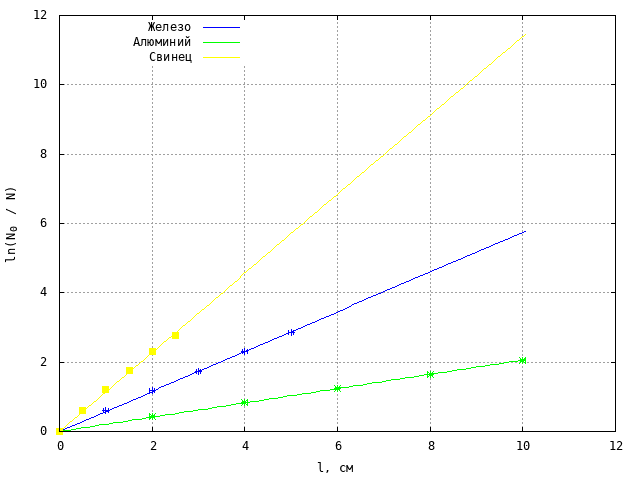
\includegraphics[width = 14cm, height = 10cm]{plot1.png}
	\caption{График зависимости $ln(N_0 / N) = f(l)$ для железа, свинца и алюминия}
\end{figure}
\begin{align*}
	\mu_\text{Fe} &= \left(0.575 \pm 0.003\right) \, \text{см}^{-1} \\
	\mu_\text{Al} &= \left(0.2062 \pm 0.0006\right) \, \text{см}^{-1} \\
	\mu_\text{Pb} &= \left(1.140 \pm 0.013\right) \, \text{см}^{-1} \
\end{align*}

\par
	Согласно приложенной таблицы линейных коэффициентов поглощения $\gamma$-лучей в различных веществах средняя энергия $\gamma$-квантов, испускаемых источником
\[
	E_\gamma \approx 0.7 \, \text{МэВ}
\]

\end{document}